\begin{figure}[H]
\centering
\includegraphics[page=6,width=0.48\textwidth]{\FCNCFigures/tthML/showFake/faketau/postfit/NOMINAL_closureTest/lowBDT_reg1l1tau1b1j_ss_vetobtagwp70_highmet/lep_pt_0.pdf}
\includegraphics[page=6,width=0.48\textwidth]{\FCNCFigures/tthML/showFake/faketau/postfit/NOMINAL_closureTest/lowBDT_reg1l1tau1b2j_ss_vetobtagwp70_highmet/lep_pt_0.pdf}

\includegraphics[page=6,width=0.48\textwidth]{\FCNCFigures/tthML/showFake/faketau/postfit/NOMINAL_closureTest/lowBDT_reg1l1tau1b2j_os_vetobtagwp70_highmet/lep_pt_0.pdf}
\includegraphics[page=6,width=0.48\textwidth]{\FCNCFigures/tthML/showFake/faketau/postfit/NOMINAL_closureTest/lowBDT_reg1l1tau1b3j_os_vetobtagwp70_highmet/lep_pt_0.pdf}


\caption{ The data-MC comparison of lepton $\pt$ in the low BDT score regions(BDT score < -0.6) for ABCD closure test after the fake tau correction and QCD estimation. }
\label{fig:closuretest}
\end{figure}
